\begin{thesischapter}{2} {Análisis, diseño e implementación del Juego Serio}
    \subthesischapter{Arquitectura del sistema}
    Antes de adentrarnos en los aspectos técnicos de la ingeniería de software, es esencial comprender el contexto en 
    el que se desarrolla la aplicación. En este caso, se trata de un sistema de rehabilitación neuromuscular lógicamente 
    separado por 2 componentes autónomos e independientes, que interactúan entre si: juego serio(cliente) y pedal 
    motorizado(servidor), ver figura \ref{fig: system}. Los dispositivos de pedaleo ofrecen ventajas significativas en la 
    rehabilitación de pacientes con trastornos neurológicos, como la mejora de las funciones motoras y la inducción de 
    neuroplasticidad beneficiando asi que dichos componentes se encuentran organizados hacia la realización de un objetivo, el desarrollo 
    de la capcidad física tanto para usuarios sanos como para enférmos. A continuación se precisan las 
    características detalladas de cada uno.

    \vspace{10pt}    
    
    \begin{figure}[ht]
        \centering
        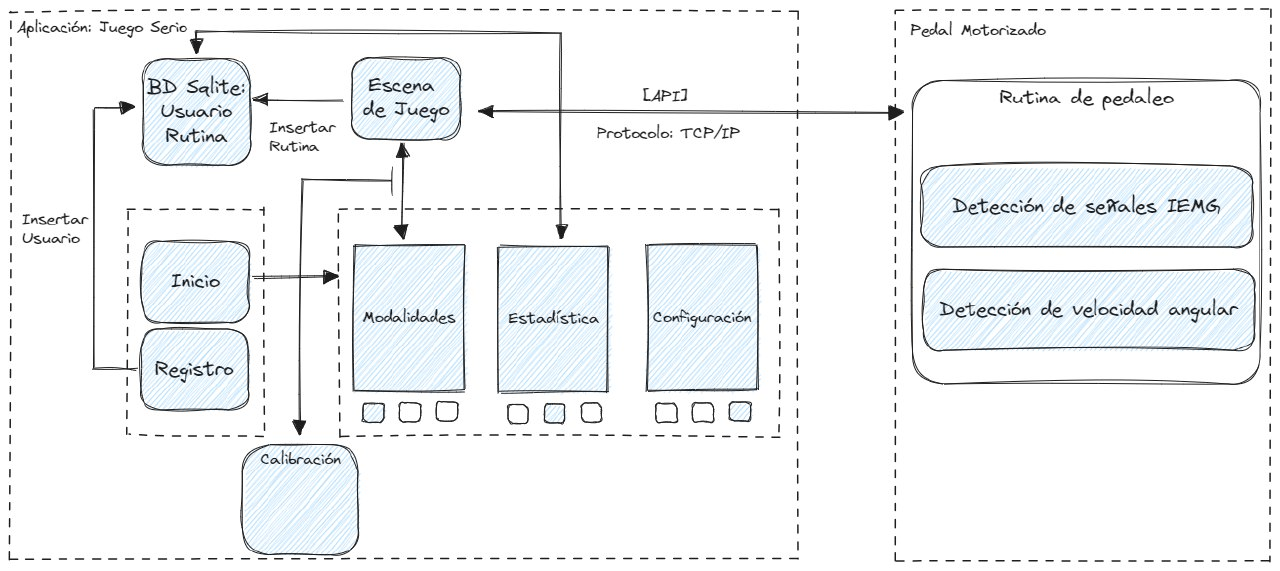
\includegraphics[scale=0.3]{images/system.jpg}
        \caption{Diagrama del sistema}
        \label{fig: system}
    \end{figure}

    La aplicación de juego serio (cliente) es responsable de:
    \begin{itemize}
        \item Recibir y procesar las señales del arduino incluido en el pedal para ser utilizadas tanto en la 
              animación de la escena como en la estadística .
        \item La carga y procesamiento de las escenas y los paradigmas de las rutinas junto a la lógica asociada. 
        \item Procesar los eventos registrados durante la realización de la rutina y devolver un análisis sobre los resultados.
        \item Gestionar los datos del usuario.
    \end{itemize}

    \vspace{10pt}
    El pedal motorizado (servidor) es responsable de:
    \begin{itemize}
        \item Capturar a partir de electrodos las señales EMG del cuerpo humano correspondientes al tren inferior.
        \item Capturar la velocidad angular en los pedales.
        \item Enviar en tiempo real los datos capturados a cualquier aplicación de juego serio sincronizada.
    \end{itemize}
    
    \subthesischapter{Requisitos del Juego Serio}
    Un requisito es una restricción que el sistema debe cumplir. Tiene como propósito expresar un comportamiento o propiedad que 
    el sistema debe poseer~\cite{jacobson2000uml}. El objetivo esencial de un requisito es el de definir un comportamiento específico 
    de manera clara y comprensible tanto para los intermediarios como para el equipo de desarrollo. Pueden clasificarse en funcionales 
    y no funcionales.

    \subsubthesischapter{Requisitos funcionales }
    La integración de tecnologías de pedalo en el campo de la rehabilitación neuromuscular ha abierto nuevas oportunidades 
    para mejorar la calidad y eficacia de las terapias. En particular, los juegos serios han demostrado ser una herramienta 
    efectiva para motivar a los pacientes durante el proceso de rehabilitación. Debido a dicha necesidad fue necesario   
    el desarrollo de una aplicación android que cumpliera con los siguientes requerimientos funcionales:

    \begin{enumerate}
        \item Iniciar sesión en el sistema
        \item Registrarse en el sistema
        \item Eliminar cuenta de usuario en el sistema
        \item Editar los datos del personales
        \item Cerrar sesión
        \item Enviar datos al pedal
        \item Recibir datos del pedal
        \item Establecer comunicación con el pedal
        \item Finalizar comunicación con el pedal
        \item Detener o reanudar el juego
        \item Guardar registro de comportamieto en archivo logs
        \item Iniciar juego
    \end{enumerate}
    \subsubthesischapter{Requisitos no funcionales}
    Los requisitos no funcionales son propiedades o cualidades que el producto debe tener. Enuncian los requisitos del sistema que no pueden ser expresados como funcionalidades en respuesta a alguna acción de un usuario. Algunas de las categorías más comunes para clasificar un requisito no funcional son las siguientes: usabilidad, desempeño o rendimiento, robustez, fiabilidad, seguridad, hardware y despliegue.
    
    \vspace{10pt}
    En nuestro caso se identificaron los siguientes requisitos no funcionales:
    
    \vspace{10pt}
    \underline{Requisitos de usabilidad}
    \begin{itemize}
        \item La interfaz de trabajo del usuario con la herramienta deberá ser simple, interactiva e intuitiva y deberá notificar los diferentes errores que se produzcan durante su ejecución.
    \end{itemize}

    \underline{Requisitos de escalabilidad}
    \begin{itemize}
        \item La aplicación debería ser capaz de escalar para manejar un aumento en el número de usuarios o la cantidad de datos sin perder rendimiento.
    \end{itemize}

    \underline{Interoperabilidad }
    \begin{itemize}
        \item Si la aplicación interactúa con otros sistemas, debe ser capaz de hacerlo de manera eficiente y sin problemas 
    \end{itemize}

    \subthesischapter{Definición de los casos de usos}
    \subsubthesischapter{Identificación de los actores}
    Los actores no son parte del sistema, pero sí pueden intercambiar información con él, ellos representan un rol que juegan una o varias personas, un equipo o un sistema automatizado. En la aplicación
    de juego serio se identificaron los siguientes actores:

    \begin{table}[ht]
        \centering
        \begin{tabularx}{\textwidth}{|l|X|}
            \hline
            \textbf{Actores} & \textbf{Descripción} \\\hline
            Usuario & Individuo que interactúa con el sistema para hacer uso de una rutina de entrenamiento
            como medio de rehabilitación, diversión o entrenamiento físico \\\hline
            Sistema & Es la misma aplicación que en determinadas ocasiones ejecuta funcionalidades automáticamente producto de la interacción con el pedal. \\\hline
        \end{tabularx}
        \label{tab: actores}
        \caption{Descripción de actores}
    \end{table}


    \vspace{100pt}
    \subsubthesischapter{Identificación de los casos de usos}    
    El actor del sistema, o sea, quien interactúa con la aplicación, en este trabajo, es el usuario del sistema, encargado 
    de utilizar todas las funciones del mismo. Cada forma en que los actores usan el sistema se representa con un caso de 
    uso, como fragmentos de funcionalidad que el sistema ofrece para aportar solución a la necesidad de esta aplicación. 
    Los casos de uso que se definen para el sistema propuesto están reflejados en la cuadro: 2 con su respectivo diagrama figura: \ref{fig: use-cases}:
    
    \begin{table}[ht]
        \centering
        \begin{tabularx}{0.85\textwidth}{|c|X|c|}
            \hline
            \textbf{Casos de Uso} & \textbf{Descripción} & \textbf{Requisitos}\\\hline
            Iniciar sesión & Permite al usuario acceder al sistema & RF1\\\hline
            Registrar usuario & Permite guardar los datos de un usuario en la Base de Datos & RF2\\\hline
            Eliminar usuario & Permite eliminar la cuenta de un usuario en la Base de Datos & RF3\\\hline
            Editar datos del usuario & Permite actualizar losdatos personales del usuario en la Base de Datos & RF4\\\hline
            Cerrar sesión & Permite al usuario cerrar sesión en el sistema & RF5\\\hline
            Enviar datos al pedal & Permite a la aplicación enviar datos al pedal & RF6 \\\hline
            Recibir datos del pedal & Permite a la aplicación recibir los datos provenientes del pedal & RF7\\\hline
            Establecer comunicación & Permite establecer comunicación entre el dispositivo Android y el Pedal Motorizado & RF8\\\hline
            Finalizar Comunicación & Permite finalizar comunicación entre el dispositivo Android y el Pedal Motorizado & RF9\\\hline
            Pausar/Reanudar juego & Permite pausar la etapa actual del juego & RF10\\\hline
            Guardar logs & Permite almacenar los hechos ocurridos en el sistema en ficheros de logs & RF11\\\hline
            Iniciar juego & Permite dar inicio a la rutina de entrenamiento & RF12\\\hline
            %Iniciar juego rutina libre & Permite dar inicio a la rutina de entrenamiento libre \\\hline
            %Iniciar juego rutina resistido & Permite dar inicio a la rutina de entrenamiento resistido \\\hline
        \end{tabularx}
        \label{tab: rf}
        \caption{Requisitos funcionales del sistema}
    \end{table}
    
    \begin{figure}[ht]
        \centering
        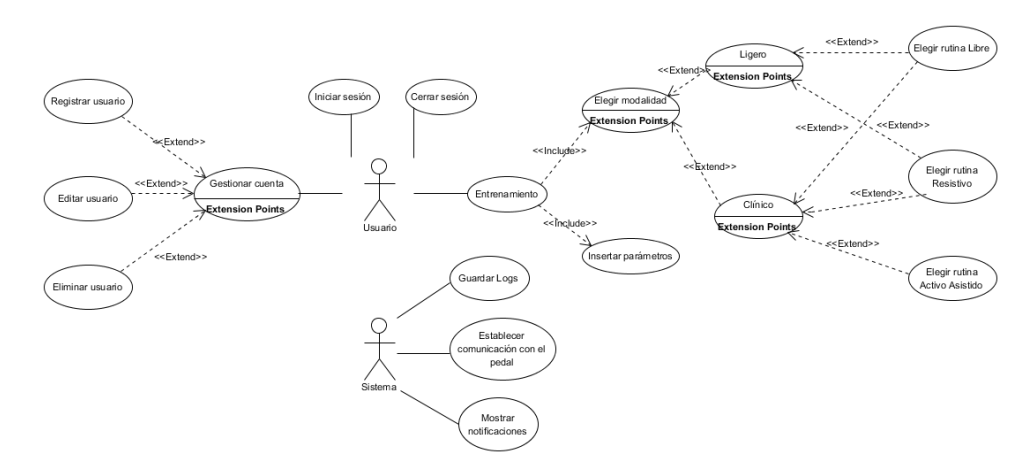
\includegraphics[scale=0.4]{images/casosdeuso.png}
        \caption{Diagrama de Casos de Uso}
        \label{fig: use-cases}
    \end{figure}

    \subthesischapter{Realización de los casos de uso}
    La realización de los casos de uso en el análisis es una colaboración que describe cómo se lleva a cabo y ejecuta un caso de uso determinado en término de las clases del análisis y de sus objetos en interacción, por lo tanto, se centra en los requisitos funcionales. A 
    continuación se describirán 3 de los Casos de Usos de mayor relevancia.
    
    
    \begin{center}
        \begin{table}
            \begin{tabularx}{0.95\textwidth}{|X|X|}
                \hline
                \textbf{Caso de uso:} & Establecer comunicación con el pedal \\\hline
                \textbf{Actores:} &  Sistema \\\hline
                \multicolumn{2}{|X|}{        
                \begin{minipage}[t]{0.925\columnwidth}
                    \textbf{Descripción:} \\
                    El caso de uso se inicia cuando se necesita registrar una nueva venta de producto, el dependiente introduce nombre, identificador, fecha, cantidad, importe, si es o no de donación. Se comprueba la disponibilidad de la oferta. Si no hay suficiente cantidad finaliza el caso de uso. En caso contrario, el dependiente registra datos del producto, si el producto es de donación registra los datos de la entidad que asumirá el pago (ver <<curso alterno  Registro de entidad>>)y termina caso de uso.
                \end{minipage}} \\\hline
                
                \textbf{Requisitos funcionales asociados:} & RF8, RF7 \\\hline
                \textbf{Precondiciones:} & El módulo de comunicación del dispositivo móvil debe estar activado y conectado a la red wifi del pedal. \\\hline
                \textbf{Poscondiciones:} &  \\\hline
                
                1. El especialista abre la aplicación & 2. El sistema establece la conexión con el Sistema Terapéutico de Ejercicios. \\\\ &3. Termina el CU. \\\hline
            \end{tabularx}

            \caption{Descripción del CU: Establecer comunicación con el pedal}
        \end{table}
    \end{center}
    
    
    
    \subsubthesischapter{Diagrama de clases}



    % DATABASE --------------------------------------
    \subthesischapter{Diseño de la base de datos}
    Las bases de datos son, en esencia, estructuras de datos que funcionan según una serie de reglas que nosotros mismos 
    definimos. Nos liberan del ajetreo de la microgestión, pero nos dan la libertad de moldear los datos según nuestras 
    necesidades. Hay dos tipos famosos de bases de datos, uno se llama Lenguaje de Consulta Estructurado o SQL. Que coloca 
    los datos en forma de tablas. El otro se llama No-SQL, porque no tiene tablas ni estructura, sino que almacena los 
    datos en forma de objetos. Intuitivamente, No-SQL consume más recursos que SQL, por lo tanto, para nuestra aplicaciones 
    móviles preferimos este último.

    \vspace{10pt}
    SQLite ha sido favorecido por los desarrolladores móviles y recomendado por la documentación oficial de Android. Aún  
    Unity no ha brindado soporte oficial para crear bases de datos. Sin embargo, hemos ideado una manera de utilizar las 
    ventajas de SQLite para nuestra aplicación. 
    
    La idea utilizada fue agrupar los métodos y variables comunes en una clase. Luego extender la clase usando herencia para 
    crear implementaciones reales. Fue creada una clase de alto nivel DataBaseModel que se puede extender a otras clases, con el 
    fin de acceder a las operaciones básicas de cualquier base de datos. Llamamos a estas operaciones basicas CURD: Crear, 
    Actualizar, Leer y Borrar, ver figura \ref{fig: diagram-db}.
    \begin{figure}[ht]
        \centering
        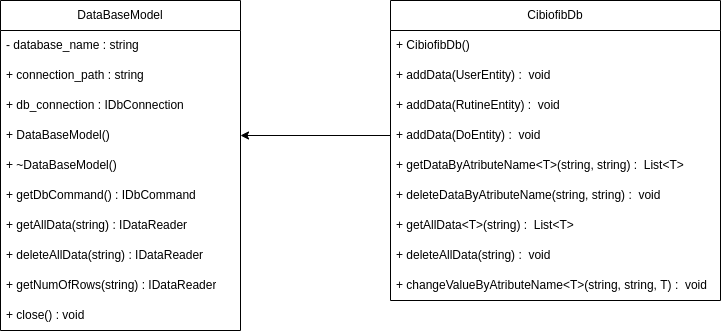
\includegraphics[scale=0.4]{images/diagram-db.png}
        \caption{Diagrama de clases Base de Datos}
        \label{fig: diagram-db}
    \end{figure}

    \vspace{10pt}
    \textbf{Requerimientos para la estructura de datos}\\
    La descripción que surge de esta fase de diseño sirve como base para especificar la estructura conceptual de la base de datos. 
    La siguiente lista describe los principales requisitos para la entrada de datos en el sistema:
    \begin{itemize}
        \item Los usuarios se identifican mediante sus valores ID\_USUARIO. Del paciente se guarda sus datos de identificación, 
        referidos en los requerimientos de registro del paciente (NOMBRE COMPLETO, GMAIL, CONTRASEÑA).
        \item Cada usuario puede configurar y ejecutar varias rutinas de entrenamiento. Las rutinas consisten de su identificador 
        único el tipo de ejercicio seleccionado y los parámetros configurados.    
    \end{itemize}
    
    \vspace{10pt}
    \textbf{Designación de los conjuntos de entidades y de relaciones}\\
    La especificación de los requisitos de datos sirve como punto de partida para la construcción
    del Modelo Entidad-Relación. Desde la especificación listada anteriormente se comienzan a
    identificar los conjuntos de entidades y relaciones, así como sus atributos:
    \begin{itemize}
        \item El conjunto de entidades usuario, con los atributos ID\_USUARIO, NOMBRE, GMAIL, CONTRASEÑA.
        \item El conjunto de entidades rutina con los atributos ID\_RUTINA, TIPO, PARÁMETROS.
        \item El conjunto de relaciones mucho a muchos de usuario a rutinas denominado tiene, es decir un usuario puede tener varias rutinas y la misma rutina puede ser ejecutada por distintos usuarios.
    \end{itemize}
    
    \vspace{10pt}
    El Diagrama de Entidad-Relación (E-R) que resulta de tales especificaciones para la descripción de los datos del sistema se presenta en la figura \ref{fig: diagram-er}.
    \begin{figure}[ht]
        \centering
        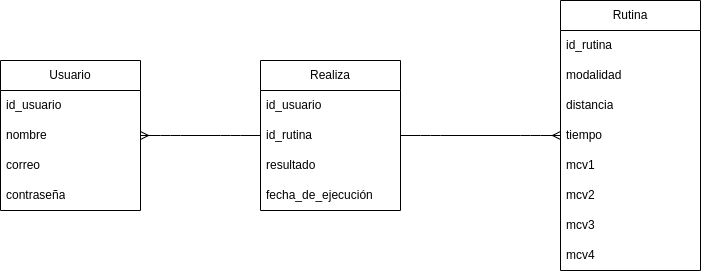
\includegraphics[scale=0.4]{images/diagram-er.png}
        \caption{Diagrama Entidad Relación}
        \label{fig: diagram-er}
    \end{figure}

    %COMUNICACION --------------------------------------------------------------
    \subsubthesischapter{Comunicación con el pedal motorizado}
    El hardware externo (pedal motorizado) posee un microcontrolador Arduino [...] programado para efectuar [....]. 
    
    
    La comunicación entre la tarjeta y la aplicación se realiza siguiendo un protocolo de comunicación establecido que 
    consta de la siguiente sintaxis: \#[COMANDO][PARÁMETROS].
    

    % \vspace{10pt}
    % \textbf{Comandos enviados por la aplicación al pedal}\\
    
    
    % \vspace{10pt}
    % \textbf{Iniciar mediciones, comando << im >>}\\
    % Envía la orden de iniciar mediciones y sigue el esquema \#im[canal1],[canal2],[canal3],[canal4],
    % [algoritmo1],[algoritmo2],[algoritmo3],[algoritmo4], donde cada canal es 1 o 0 si este se
    % encuentra activo y algoritmo indica el algoritmo a emplear en el cálculo de la MCV.
    
    % \vspace{10pt}
    % Ejemplo: \#im1,0,1,0,1,1,2,2,
    % Inicia las mediciones por los canales 1 y 3 Con el algoritmo 1 para el canal 1 y el algoritmo 2 para el canal 3, para
    % los canales no seleccionados se omite el tipo de algoritmo seleccionado.
    
    % \vspace{10pt}
    % \textbf{Parar mediciones, comando << sm >>}\\
    % Envía la orden de parar las mediciones.

    % \vspace{10pt}
    % \textbf{Iniciar juego, comando << ig >>}\\
    % Establece el inicio del juego y sigue el siguiente esquema: 
    % \#ig[velocidad], [tiempo], [canal1], [canal2], [canal3], [canal4], donde:

    % \vspace{5pt}
    %  Velocidad: Establece el porciento de velocidad a la que se realizará el ejercicio. Puede tomar valores de 1 a
    % 100.

    % \vspace{5pt}
    %  Tiempo: Establece el tiempo en minutos durante el cual se realizará el ejercicio. Puede tomar valores de 1 a 60.
    %  Descanso: Establece el tiempo en minutos de descanso entre series. Puede tomar valores de 1 a 60.
    %  Canal[1-4]: Establece con qué canales se va trabajar. Pueden tomar valores 0/1 siendo el valor 1 especificando que dicho canal específico estará siendo usado.
    %  Tipo: Establece el tipo de rutina a ejecutar.
    %  
    % Ejemplo: \#ir50,10,5,20,1,1,0,0,1,80,0,

    % En este ejemplo se establece una parametrización donde se realiza el ejercicio al 50% de velocidad, durante 10
    % minutos, con 5 minutos de descanso entre series, se realizarán 20 series, solo se escucharán los canales 1 y 2 y la
    % rutina será activa/asistida en un 80\%.

    % \vspace{10pt}
    % \textbf{Parar juego, comando << sg >>}\\
    % Envía la orden de parar la ejecución de la rutina.
    
    % \vspace{10pt}
    % \textbf{Pausar rutina, comando << pr >>}\\
    % Envía la orden de pausar la rutina.

    
    % \vspace{10pt}
    % \textbf{Continuar rutina, comando << cr >>}\\
    % Envía la orden de continuar con la ejecución de la rutina.
    

    % \vspace{10pt}
    % \textbf{Activar/Desactivar canales, comando << ch >>}
    % Envía la orden de activar o desactivar los canales de mediciones y sigue el siguiente esquema: \#ch[canal],[acción], donde:
    %  Canal: Establece el canal sobre el que se va a realizar la acción.
    %  Acción: Establece si se va a activar o desactivar dicho canal.
    
    % \vspace{10pt}
    % \textbf{Transmitir mediciones, comando << tm >>}
    % Envía la orden de transmitir mediciones, se envía en caso de que la respuesta del comando correspondiente al
    % estado del pedal sea diferente a << nada >>.
    
    
    % \vspace{10pt}
    % \textbf{Máxima contracción voluntaria, comando << mc >>}
    % Establece las acciones correspondientes al trabajo con la MCV y sigue el siguiente esquema: \#mc[canal],
    % [acción], donde:
    %  Canal: Establece el canal sobre el que se va a realizar la acción.
    %  Acción: Establece la acción, esta puede ser:
    % o Iniciar iteración cálculo de MCV
    % o Detener iteración Cálculo de MCV
    % o Aceptar valor de iteración del cálculo de MCV
    % o Rechazar valor de iteración del cálculo de MCV

    % \vspace{10pt}
    % \textbf{Línea base, comando << lb >>}
    % Establece las acciones correspondientes al trabajo con la Línea Base y sigue el siguiente esquema: \#lb[canal],
    % [acción], donde:
    %  Canal: Establece el canal sobre el que se va a realizar la acción.
    %  Acción: Establece la acción, esta puede ser:
    % o Iniciar iteración cálculo de Línea Base
    % o Detener iteración Cálculo de Línea Base
    % o Aceptar valor de iteración del cálculo de Línea Base
    % o Rechazar valor de iteración del cálculo de Línea Base

    % \vspace{10pt}
    % \textbf{Requerir valores de máxima contracción voluntaria y línea base << rv >>}\\
    % Establece el pedido de los valores finales de máxima contracción voluntaria y línea base para los canales y sigue el
    % siguiente esquema: \#rv[lb1],[lb2],[lb3],[lb4],[mc1],[mc2],[mc3],[mc4], donde:

    % lb1-4: requiere el valor de línea base para dicho canal, puede tomar valores de 0 o 1 si se pide o no dicho valor.
    % mc1-4: requiere el valor de máxima contracción voluntaria para dicho canal, puede tomar valores de 0 o 1 si
    % se pide o no dicho valor.
    % Ejemplo: \#rv1,0,0,1,0,1,1,0,
    % Se solicitan los valores de línea base para los canales 1 y 4 y el valor de la máxima contracción voluntaria para los
    % canales 2 y 3.

    % \vspace{10pt}
    % \textbf{Parada general, comando << sg >>}
    % Envía la orden de parada general al pedal. Usado como parda de emergencia.
    
    % \vspace{10pt}
    % \textbf{Estadísticas, comando << es >>}
    % Pide al Sistema Terapéutico de Ejercicios las estadísticas del ejercicio realizado



    % \vspace{20pt}
    % Para lograr el funcionamiento del software en tiempo real donde se pudiera mantener la
    % comunicación con la tarjeta y a la vez atender los eventos de los botones de la interfaz cada
    % vez que son oprimidos, fue necesario funciones avanzadas de Labwindows que permitieran
    % crear y habilitar un hilo paralelo independiente de la función principal ver figura \ref{fig: diagram-protocol}.

    \begin{figure}[ht]
        \centering
        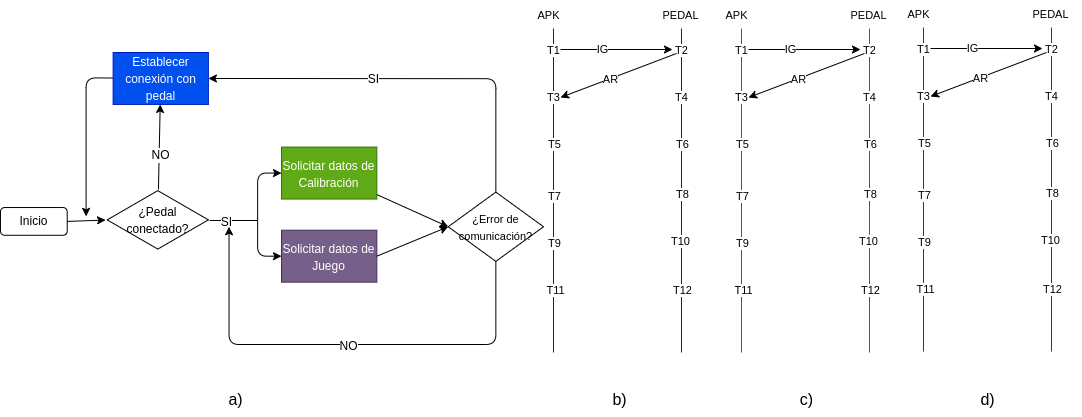
\includegraphics[scale=0.32]{images/diagram-protocol.png}
        \caption{a)~Diagrama de flujo del protocolo de comunicación b)~Protocolo de inicialización}
        \label{fig: diagram-protocol}
    \end{figure}

    \subsubthesischapter{Entornos de entrenamiento}
    Se crearon distintos entornos de entrenamiento correspondientes a las modalidad Ligero y Clínico. Para cada uno de 
    estos se tuvieron las siguientes consideraciones.

    \vspace{10pt}
    \textbf{Configuración del entrenamiento} \\ 
    ----- menu de parámetros ----------

\end{thesischapter}